% details-of-test-conditions.tex

\chapter{CART3D Results}

\section{Engine-On Plume Check}
-simulate engine-on conditions to check that the plumes do not adversely affect the tail of the vehicle (justify that I can just remove engines/boattail)

-Mach 5,7,9 at 50kPa

\section{CART3D Results}
-include mesh here

\begin{figure}
	\centering
	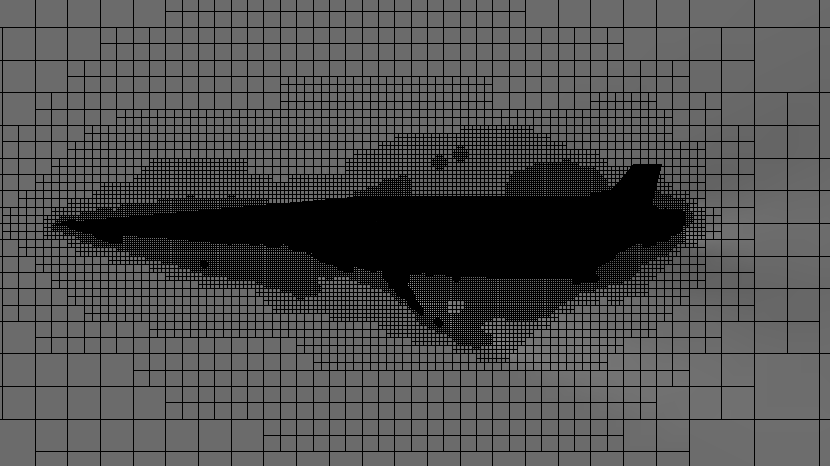
\includegraphics[width=0.7\linewidth]{figures/3_vehicle_design/M3AoA6GRID}
	\caption{}
	\label{fig:M3AoA6GRID}
\end{figure}

		\begin{figure}
			\centering
			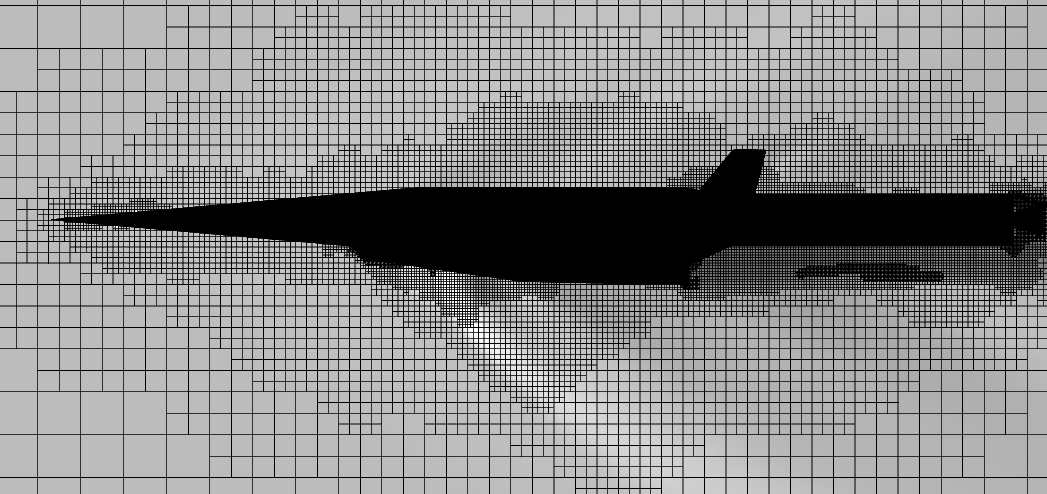
\includegraphics[width=0.7\linewidth]{figures/3_vehicle_design/CARTmesh}
			\caption{ Mesh generated by CART3D around the SPARTAN and first stage vehicles.}
			\label{fig:CARTmesh}
		\end{figure}
		
		
		
		\begin{figure}
			\centering
			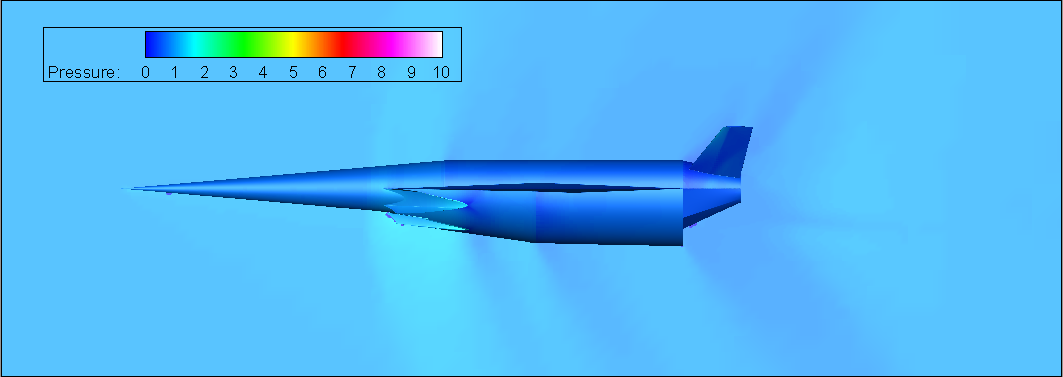
\includegraphics[width=0.9\linewidth]{figures/3_vehicle_design/M1p1AoA6}
			\caption{CART3D flow result for the SPARTAN, at Mach 1.1, 6$^\circ$ angle of attack.}
			\label{fig:M1}
		\end{figure}
		\begin{figure}
			\centering
			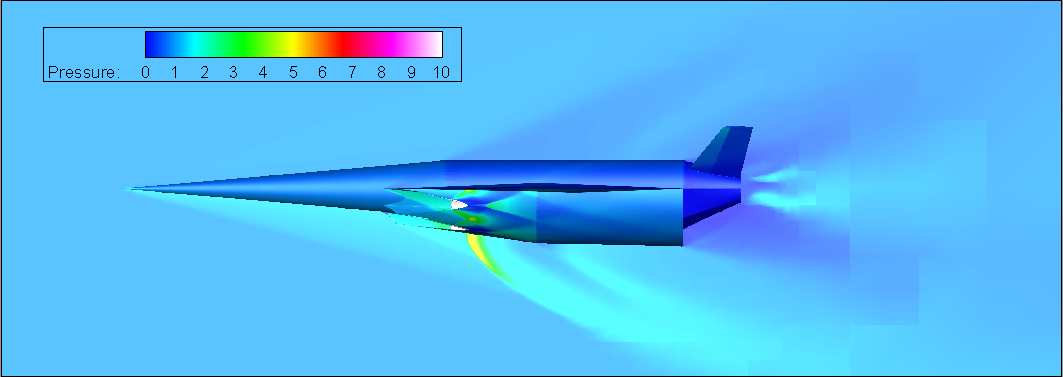
\includegraphics[width=0.9\linewidth]{figures/3_vehicle_design/M3AoA6}
			\caption{CART3D flow result for the SPARTAN, at Mach 3, 6$^\circ$ angle of attack.}
			\label{fig:M3AoA6}
		\end{figure}